\documentclass{report}
\usepackage[margin=0in,paperwidth=5.2in,paperheight=1.25in]{geometry}
\usepackage{tikz}
\usetikzlibrary{calc}
\usetikzlibrary{decorations.pathreplacing}
\pagestyle{empty}
% \hoffset -0.4in
% \voffset 0.75in
\begin{document}
% \begin{center}
%     \begin{tikzpicture}[scale=2]
%         \draw[decorate,decoration={brace,amplitude=5pt,mirror}](0,-1) -- (0,-2) node[pos=0.5,left,xshift=-5pt]{$IP=[2,6,3,1,4,8,5,7]$};
%         \draw[decorate,decoration={brace,amplitude=5pt,mirror},yshift=-10pt](0,-2) -- (0,-3) node[pos=0.5,left,xshift=-5pt]{$IP^{-1}=[4,1,3,5,7,2,8,6]$};
%         \foreach \i/\f in{1/4,2/1,3/3,4/5,5/7,6/2,7/8,8/6}{
%             \pgfmathparse{int(\i+1)}\let\sl=\pgfmathresult;
%                 \node[anchor=south] at (\i/2,-1) {$b_\i$};
%                 \node[anchor=north] at (\f/2,-2) {$b_\i$};
%                 \draw[->,dashed](\i/2,-1) to[out=270,in=90] (\f/2,-2);
%         };
%         \foreach \i/\f in{1/4,2/1,3/3,4/5,5/7,6/2,7/8,8/6}{
%             \pgfmathparse{int(\i+11)}\let\sl=\pgfmathresult;
%                 \node[anchor=north,yshift=-16pt] at (\i/2,-3) {$b_\i$};
%                 \draw[->,yshift=-8pt,dashed](\f/2,-2) to[out=270,in=90] (\i/2,-3);
%         };
%     \end{tikzpicture}
% \end{center}

% \pagebreak

\begin{center}
    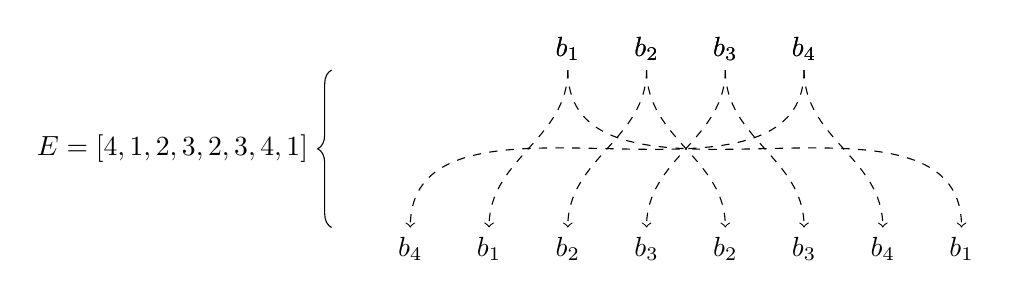
\begin{tikzpicture}[scale=2]
        \draw[decorate,decoration={brace,amplitude=5pt,mirror}](0,-1) -- (0,-2) node[pos=0.5,left,xshift=-5pt]{$E=[4,1,2,3,2,3,4,1]$};
        \foreach \i/\f in{1/2,1/8,2/3,2/5,3/4,3/6,4/1,4/7}{
            \pgfmathparse{int(\i+1)}\let\sl=\pgfmathresult;
                \node[anchor=south] at (1+\i/2,-1) {$b_\i$};
                \node[anchor=north] at (\f/2,-2) {$b_\i$};
                \draw[->,dashed](1+\i/2,-1) to[out=270,in=90] (\f/2,-2);
        };
    \end{tikzpicture}
\end{center}


\end{document}